
%
% raspberry p3 spec: https://www.raspberrypi.org/magpi/raspberry-pi-3-specs-benchmarks/

\section{Embedded Computing Platform Comparison}\label{sec:comparison}

In this section, we compare three computing platforms---the Raspberry
Pi 3, the Intel UP~\footnote{http://www.up-board.org/up/} and NVIDIA
Jetson
TX2~\footnote{http://www.nvidia.com/object/embedded-systems-dev-kits-modules.html}---from
the point of view of supporting vision-based end-to-end deep learning
based autonomous vehicles. 
Table~\ref{tbl:platforms} shows architectural features of the three
platforms~\footnote{The GPUs of the Raspberry Pi 3 and Intel
  Up are not used in evaluation due to the lack of software (TensorFlow)
support. Also, the two Denver cores in Tegra TX2 are not used in
evaluation due to TensorFlow issues.}.
  
Our basic approach is to use the same DeepPicar software, and repeat
the experiments in Section~\ref{sec:evaluation} on each hardware
platform and compare the results. 
For Tegra TX2, we have two different system configurations,
which differ in whether TensorFlow is configured to use its GPU or
only the CPU cores. Thus, the total four system configurations are
compared.

\begin{figure}[h]
  \centering
  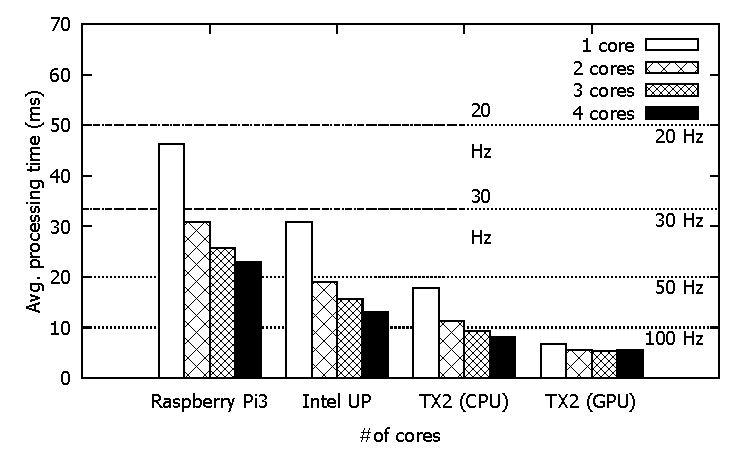
\includegraphics[width=.45\textwidth]{figs/compare_core}
  \caption{Average control loop execution time.} 
  \label{fig:sys_core}
\end{figure}

Figure~\ref{fig:sys_core} shows the average control loop completion
timing of the four system configurations we tested as a function of
the number of CPU cores used.
First, both the Intel UP and Tegra TX2 exhibit superior performance when
compared with the Raspberry Pi 3. 
When all four CPU cores are used, the Intel UP is 2.53X faster than
the Pi 3, while TX (CPU) and TX (GPU) are 3.6X and 7.6X times faster,
respectively, than the Pi 3. 
As a result, they are all able to satisfy the 50 ms 
WCET by a clear margin,
%%  (in the worst case, the UP Board would 
%% still meet it by $\sim$20 ms) --> where's the data showing this?
and, in case of TX2, 50 Hz or even 100 Hz real-time control is
feasible with the help of its GPU. Another observation is that TX2
(GPU) does not change much, as most of the neural network computation
is done at the GPU.

\begin{figure}[h]
  \centering
  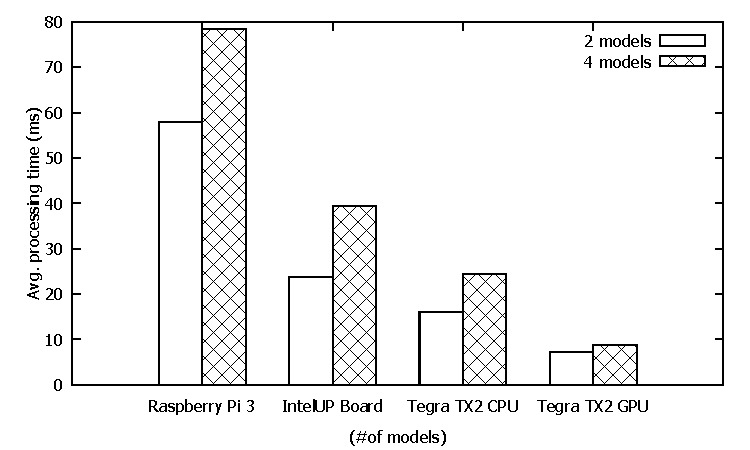
\includegraphics[width=.45\textwidth]{figs/compare_model}
  \caption{Average control loop execution time when multiple DNN
    models are co-scheduled. }
  \label{fig:sys_model}
\end{figure}

The UP Board and TX2 also perform much better when multiple DNN models
are co-scheduled. Figure~\ref{fig:sys_model} shows the results of the
multi-model co-scheduling experiment. Once again, they can comfortably
satisfy 20 Hz real-time performance for all of the co-scheduled DNN control
loops, and in case of TX 2 (GPU), 100 Hz real-time control is still
feasible. Given that the GPU must be shared among the co-scheduled DNN
models, the result suggests that TX2's GPU has sufficient capacity to
accomodate multiple instances of the DNN model we tested.

%% to complete control loops in a fraction of the time when compared to 
%% the Pi. Furthermore, both of the platforms satisfied the 50 ms WCET 
%% in all experiments, while the Raspberry Pi 3 was unable to do so. As 
%% such, the UP Board and TX2 display greater potential for the 
%% simultaneous execution of multiple models during self-driving 
%% operation, while the Raspberry Pi 3 would struggle to do so.

\begin{figure}[h]
  \centering
  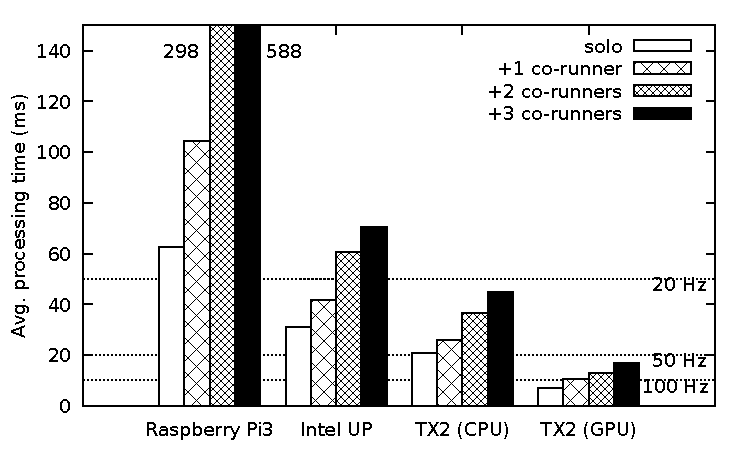
\includegraphics[width=.45\textwidth]{figs/compare_benchmark}
  \caption{Average control loop execution time in the presence of an
    increasing number of memory intensive applications on idle CPU cores.}
  \label{fig:sys_bench}
\end{figure} 

Finally, we compare the effect of co-scheduling memory bandwidth
intensive synthetic benchmarks on the DNN control loop timing. 
Figure~\ref{fig:sys_bench} shows the results.
As discussed in 
Section~\ref{sec:eval-memhog}, we observed dramatic execution time
increases, up to 9.4X, in Raspberry Pi 3 as we increased the number of
co-scheduled tasks. We also observe increased control loop execution
timing in Intel Up and TX2, but the degree of the increase is not as
dramatic as the Pi3. Compared to their respective solo timings (i.e.,
the model runs on a single core in isolation), Intel UP suffers up to
2.3X execution time increase; TX2 (CPU) and TX2 (GPU) suffer up to
2.2X and 2.5X increase, respectively. This is somewhat suprising
because Raspberry Pi 3's cores are in-order architecture based while
the cores in Intel Up and NVIDIA TX2 are out-of-order architecture
based, and that the memory intensive tasks on out-of-order cores can
generate more memory traffic. We suspect that this is because the
memory subsystems in the Intel UP and TX2 platforms provide higher
bandwidth and fairness than the memory subsystem of the Pi 3.

Another intersting observation is that TX2 (GPU) also suffers
considerable execution time increase (2.5X) despite the fact that the
co-scheduled synthetic tasks do not utilize the GPU. In other words,
the DNN model has dedicated access to the GPU. This is, however, a
known characteristic of integrated CPU-GPU architectue based
platforms where both CPU and GPU share the same memory
subsystem~\cite{Ali2017}. As a result, TX2 (GPU) fails to meet the
10ms deadline for 100 Hz control that would have been feasible if
there was no contention between the CPU cores and the GPU.

%% experienced a change in their inferencing times, but the increases 
%% were not as drastic as is seen by the Raspberry Pi 3. in the worst 
%% case, both the UP Board and TX2 (CPU only and GPU) produced times 
%% that were over two times as large, whereas the Raspberry Pi 3 output 
%% times that were around 10 times greater. The Intel UP Board was 
%% successful in completing inferencing operations in under 50 ms when 
%% benchmarks were run on a maximum of 2 cores, and the TX2 was 
%% successful in all experiments irrespective of the computing resources 
%% utilized. Comparetively, both performed better than the Raspberry Pi 
%% 3 which failed to meet its deadlines when any benchmark was 
%% introduced. As such, it can be concluded that the Intel UP Board 
%% would be more capable of running computationally heavy processes 
%% during autonomous driving, and that the Pi wouldn't be able to do the 
%% same.

In summary, we find that today's embedded computing platforms, even as
inexpensive as a Raspberry Pi 3, are powerful enough to support
vision and end-to-end deep learning based real-time control
applications. Furthermore, availability of CPU cores and GPU on these
platforms allow consolidating mutiple deep neural network based AI
workloads. However, shared resource contention among these diverse
computing resources remains an important issue that must be understood
and controlled, especially for safety-critical applications.

%% the comparison of the real-time capabilities of three embedded 
%% computing platforms, we found that the Raspberry Pi 3 performed the 
%% worst. When compared to the Intel UP Board and the NVIDIA Tegra TX2, 
%% control loops on the Pi were shown to take noticably longer to 
%% complete, regardless of the number of cores utilized or the number of 
%% neural network models run simultaneoulsy. The difference was even 
%% more noticeable in the the addition of computationally heavy 
%% synthetic benchmarks that had a much more dire effect on the Pi. In 
%% the worst case, an average control loop on the Pi took an abnormally 
%% long amount of time to finish. Compared to the TX2 with GPU support, 
%% those times were 34.8X times greater. From this, we find that the UP 
%% Board and Tegra TX2 are superior platforms for real-time CNN 
%% operations. However, due to the Pi's ability to satisfy the 50 ms 
%% WCET in some experiments, we conclude that the Raspberry Pi 3 is 
%% feasible for autonomous research.



